% 第 3 章 Using GUI Assistant Tools
\bichapter{使用 GUI 助手工具}{Using GUI Assistant Tools}
\label{chap:gui-assist}

IC Compiler II GUI 提供多种助手，例如任务助手（Task Assistant）、线网助手（Net Assistant）、管脚助手（Pin Assistant）和设计助手（Design Assistant），用来管理设计中的不同对象。例如，任务助手把常用命令归集到不同流程中，以支持设计规划（design planning）、时序分析（timing analysis）、布局（placement）以及其他流程。GUI 助手工具可以简化设计过程。

本章说明如何使用这些 GUI 工具，包括以下主题：
\begin{itemize}
  \item 使用任务助手
  \item 使用设计助手
  \item 用相对位置约束工具设置约束
  \item 使用网表追踪器
  \item 使用布线轨道助手
\end{itemize}

\section{使用任务助手}
\subsection*{Using the Task Assistant}

任务助手便于浏览设计规划及其他流程，并执行单项任务来完成设计。以下几节说明任务助手的主要功能。

\subsection{启动 Tasks 工具栏与任务助手}
\subsubsection*{Starting the Tasks Toolbar and Task Assistant}

要打开 Tasks 工具栏，从菜单选择 \textbf{View > Toolbars > Tasks}。工具在版图视图（layout view）右侧显示任务面板，见图~\ref{fig:gui-31}。

\begin{figure}[htbp]
\centering
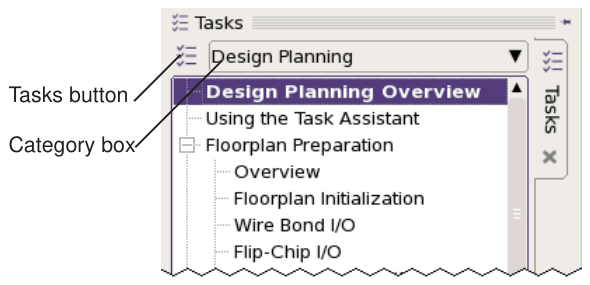
\includegraphics[width=0.92\textwidth]{gui-fig-031.png}
\caption{任务面板}
\label{fig:gui-31}
\end{figure}

要显示另一类别的任务列表，单击类别框（category box）右侧的向下箭头。要显示任务助手对话框，单击类别框左侧的 tasks 按钮。也可以从菜单选择 \textbf{Task > Task Assistant}。

\subsection{在任务助手对话框中浏览任务}
\subsubsection*{Navigating the Tasks in the Task Assistant Dialog Box}

任务助手对话框提供按钮，可转到任务列表中的下一项或上一项任务，也可在历史列表中后退或前进。任务助手窗口左侧是带目录（table of contents）的导航窗格（navigation pane）。在导航窗格中，选择左上角的类别，即可载入该类别的任务列表。单击导航窗格中的任一任务，即可把对应表单载入任务助手。单击导航窗格中的 [-] 图标可折叠任务子类，单击 [+] 图标可展开子类。图~\ref{fig:gui-32} 给出任务助手的部分导航功能。

\begin{figure}[htbp]
\centering
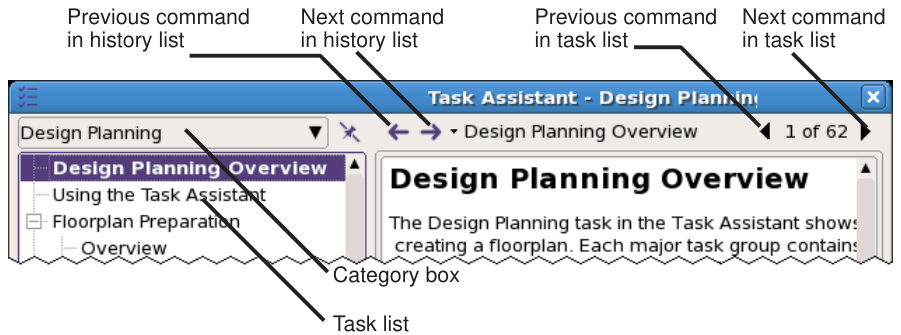
\includegraphics[width=0.92\textwidth]{gui-fig-032.png}
\caption{任务助手导航}
\label{fig:gui-32}
\end{figure}

若任务列表处于隐藏状态，如图~\ref{fig:gui-33} 所示，单击箭头将其打开，再单击图钉（pin）以显示任务列表。

\begin{figure}[htbp]
\centering
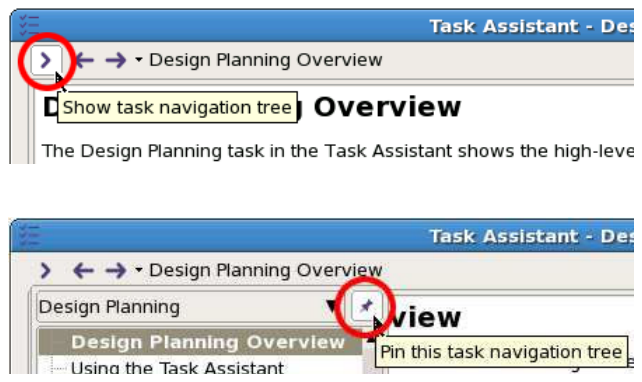
\includegraphics[width=0.92\textwidth]{gui-fig-033.png}
\caption{固定导航窗格}
\label{fig:gui-33}
\end{figure}

也可以把指针移到任务助手左侧，直到出现两条竖线。单击该竖线并向右拖动，即可显示导航栏，见图~\ref{fig:gui-34}。

\begin{figure}[htbp]
\centering
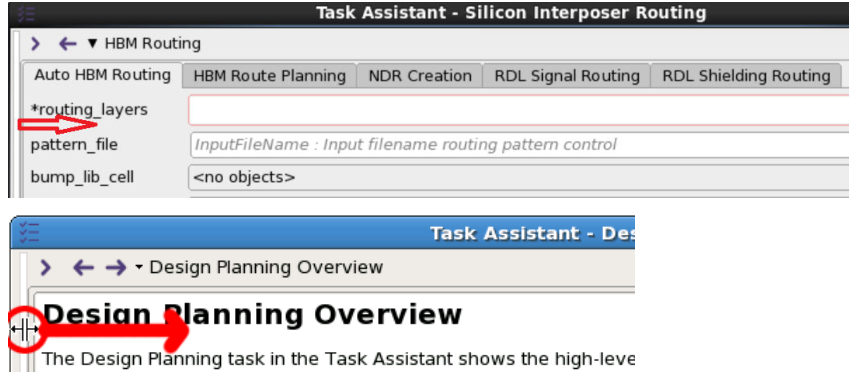
\includegraphics[width=0.92\textwidth]{gui-fig-034.png}
\caption{显示导航栏}
\label{fig:gui-34}
\end{figure}

\subsection{预览、捕获并执行命令}
\subsubsection*{Previewing, Capturing, and Issuing Commands}

填完表单数据后，查看表单底部附近的预览窗口，核对即将运行的命令，见图~\ref{fig:gui-35}。在表单中输入数据并选择选项时，该窗口会自动更新。根据某一项允许输入的数据类型，文本框可能会阻止输入不正确的信息。

\begin{figure}[htbp]
\centering
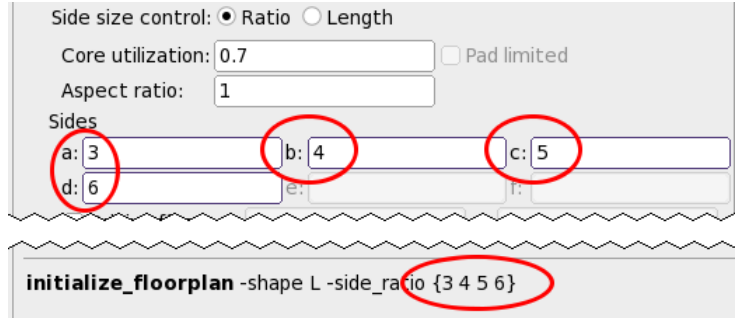
\includegraphics[width=0.92\textwidth]{gui-fig-035.png}
\caption{Tcl 命令预览窗口}
\label{fig:gui-35}
\end{figure}

改变选项或文本框中的内容，即可改变命令。单击 Script 按钮，把命令复制到 IC Compiler II GUI 版图窗口中的 Script Editor。可用 Script Editor 中的工具按需要编辑并保存该命令。

预览命令之后，单击 Apply 运行命令。若检测到命令语法有问题，工具会发出警告。若出现问题，改正表单后再试。

\subsection{使用概览页}
\subsubsection*{Using Overview Pages}

任务列表中的某些任务是在 GUI 面板中操作的。例如，Hierarchy Exploration 与 What-if Congestion Analysis 任务分别通过 GUI 中的 \textbf{View > Assistants > Hierarchy Exploration} 与 \textbf{View > Map > What-if Channel Congestion} 完成。对这些任务，任务助手提供概览页（overview page），帮助理解相应工具。图~\ref{fig:gui-36} 是 What-if Channel Congestion 的概览页。

\begin{figure}[htbp]
\centering
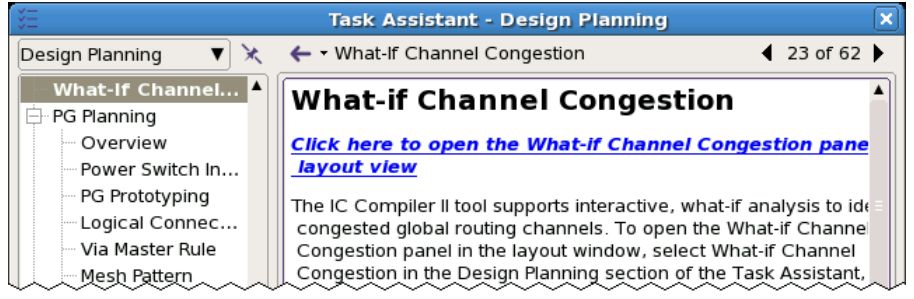
\includegraphics[width=0.92\textwidth]{gui-fig-036.png}
\caption{What-if Channel Congestion 概览页}
\label{fig:gui-36}
\end{figure}

单击页面顶部的链接，或按页面所述使用菜单命令，即可在 GUI 中打开该工具。按概览页中的说明完成该任务。

\begin{seeAlsoBox}
Hierarchy Exploration 与 What-if Channel Congestion 见第~\ref{chap:gui-dp}~章。
\end{seeAlsoBox}

\subsection{编辑表中的数据}
\subsubsection*{Editing Data in Tables}

对于设置或查看约束（constraint）信息的任务，任务助手提供可编辑的表，用于查看或修改约束数据。下列内容是 \textbf{Block Shaping > Shaping Constraints} 任务所显示的块列表，见图~\ref{fig:gui-37}。

\begin{figure}[htbp]
\centering
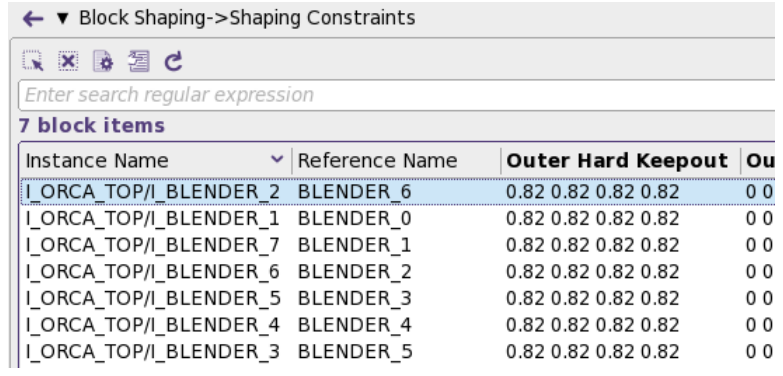
\includegraphics[width=0.92\textwidth]{gui-fig-037.png}
\caption{实例搜索}
\label{fig:gui-37}
\end{figure}

要编辑约束：
\begin{enumerate}
  \item 双击表中的一个单元格。
  \item 用 Backspace 键删除当前内容。
  \item 为该单元格输入新的约束。\\
        内容不完整或不正确时，工具以红色显示文本。有效值以黑色显示。
  \item 按 Return 键确认新值。
\end{enumerate}

编辑表单元格数据见图~\ref{fig:gui-38}。

\begin{figure}[htbp]
\centering
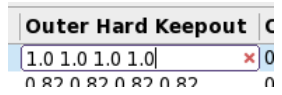
\includegraphics[width=0.92\textwidth]{gui-fig-038.png}
\caption{编辑表单元格数据}
\label{fig:gui-38}
\end{figure}

\section{使用设计助手}
\subsection*{Using the Design Assistant}

设计助手帮助在版图视图中定位并选择对象。要启动设计助手，从菜单选择 \textbf{View > Assistants > Design Assistant}，或单击 Design Assistant 按钮。界面见图~\ref{fig:gui-39}。

\begin{figure}[htbp]
\centering
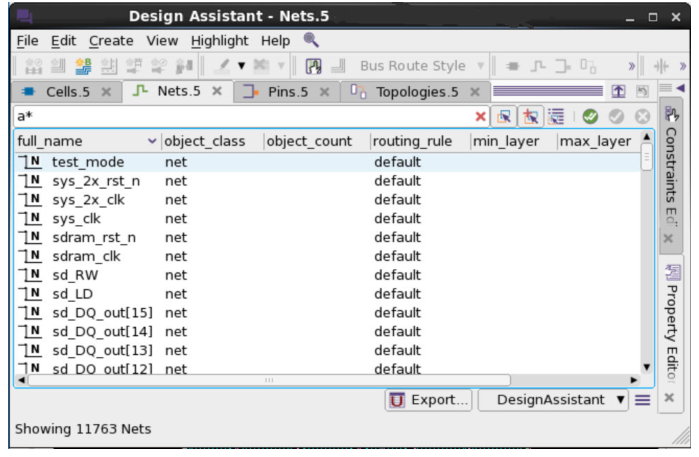
\includegraphics[width=0.92\textwidth]{gui-fig-039.png}
\caption{设计助手}
\label{fig:gui-39}
\end{figure}

以下几节说明如何使用设计助手。

\subsection{列出并选择对象}
\subsubsection*{Listing and Selecting Objects}

设计助手提供搜索框，用于列出单元、线网、管脚和拓扑（topology）对象。要填充对象列表：
\begin{enumerate}
  \item 单击 Cells、Nets、Pins 或 Topologies 选项卡。\\
        只有从上下文菜单（context menu）选择 Get Topology Plans，或使用菜单命令 \textbf{View > Topology Plans of selected} 或 \textbf{View > New Topologies} 时，Topologies 选项卡才可用。
  \item 在搜索框中输入搜索词。\\
        可以指定完整字符串、子串（substring）、通配符表达式（wildcard expression）、Tcl 命令或 Tcl 变量。例如，在搜索框中输入下列任一项，即可匹配单元 \cmd{u0\_0}、\cmd{u0\_1}、\cmd{u0\_2}、\cmd{u0\_3}（以及可能的其他单元）：
        \begin{itemize}
          \item 仅字符串：\cmd{'u'}、\cmd{'u0'} 或 \cmd{'u0\_'}
          \item 通配符：\cmd{'u0\_*'}、\cmd{'u0\_?'}
          \item Tcl 命令：
\begin{lstlisting}
get_cells "*" -filter name=~"u0*"
\end{lstlisting}
          \item Tcl 变量：\cmd{\$my\_cells}（先在工具中执行）
\begin{lstlisting}
set my_cells [get_cells "*" -filter name=~"u0*"]
\end{lstlisting}
          \item GUI 中的当前选择：\cmd{get\_selection}（在版图视图或 Hierarchy Browser 中选中 \cmd{u0\_0}、\cmd{u0\_1}、\cmd{u0\_2} 与 \cmd{u0\_3} 之后）。也可以单击搜索框右侧的 Get current selection 按钮，用所选对象填充列表。
        \end{itemize}
  \item 按 Enter。
\end{enumerate}

列表填充之后，单击列表中的单元实例，即可在版图中选中该单元。单击并拖动指针可选中多个单元；也可以在单击单元时按住 Shift 或 Control 键，把该单元加入选择。要清除选择，单击搜索框右侧的 (X)，或删除搜索框中的字符后按 Enter。

\subsection{用 Select 菜单选择对象}
\subsubsection*{Selecting Objects Using the Select Menu}

设计助手中的 Select 菜单可以快速查看并选择相关对象。用法见表~\ref{tab:gui-select-menu}。

\begin{table}[htbp]
\centering
\caption{使用 Select 菜单}
\label{tab:gui-select-menu}
\begin{tabularx}{\textwidth}{@{}X l@{}}
\toprule
要完成的操作 & 使用的功能 \\
\midrule
按对象名或搜索过滤表达式选择或高亮对象。 & Select by Name \\
把对象加入选择列表。 & Add to Selection \\
查看已选对象，例如拓扑规划、拓扑节点、拓扑起点与终点节点、拓扑边、拓扑中继器以及 MIB 拓扑实例。选择列表与工作列表的用法见第~\ref{chap:gui-toolbar}~章。 & Selection List \\
查看与所选对象相关的对象。 & Related Objects \\
清除选择列表。 & Clear \\
\bottomrule
\end{tabularx}
\end{table}

\subsection{配置设计助手中的列}
\subsubsection*{Configuring Columns in the Design Assistant}

要更改设计助手中显示的列，单击对话框底部附近属性组选择框中的向下箭头，再单击出现的列表中的一项。该列表包含此对象类型可用的属性组（attribute group），见图~\ref{fig:gui-40}。

\begin{figure}[htbp]
\centering
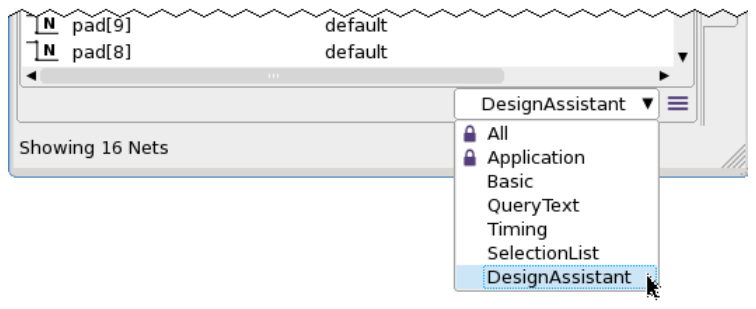
\includegraphics[width=0.92\textwidth]{gui-fig-040.png}
\caption{设计助手的属性组选择器}
\label{fig:gui-40}
\end{figure}

表中的条目可用属性组管理器（Attribute Group Manager）配置。单击对话框右下角的 Modify Attribute Group 按钮，再单击 Manage All，即可打开 Attribute Group Manager。

\begin{seeAlsoBox}
Attribute Group Manager 的用法见第~\ref{chap:gui-toolbar}~章。
\end{seeAlsoBox}

还可以对表中的列标题执行下列操作：
\begin{itemize}
  \item 单击列标题，按该列对列表中的数据排序。
  \item 再次单击该列标题，反转排序顺序。
  \item 单击列标题并把它拖到新位置，以改变列的顺序，见图~\ref{fig:gui-41}。
\end{itemize}

\begin{figure}[htbp]
\centering
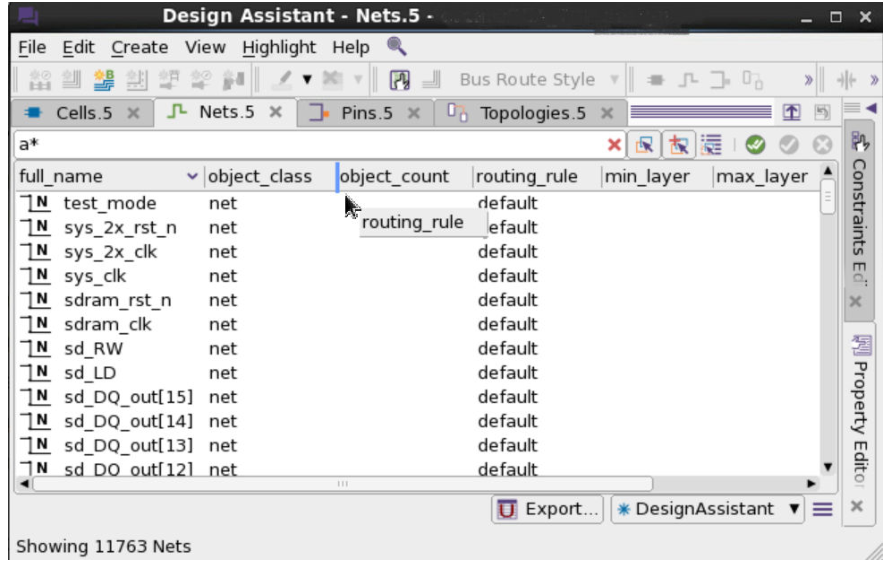
\includegraphics[width=0.92\textwidth]{gui-fig-041.png}
\caption{在设计助手中重排列}
\label{fig:gui-41}
\end{figure}

\begin{itemize}
  \item 右键单击列标题，选择 \textbf{Sort Increasing} 或 \textbf{Sort Decreasing}，对列排序。
  \item 右键单击列标题，选择 \textbf{Fit All Columns} 或 \textbf{Fit Column}，使列宽适应设计助手对话框，见图~\ref{fig:gui-42}。
\end{itemize}

\begin{figure}[htbp]
\centering
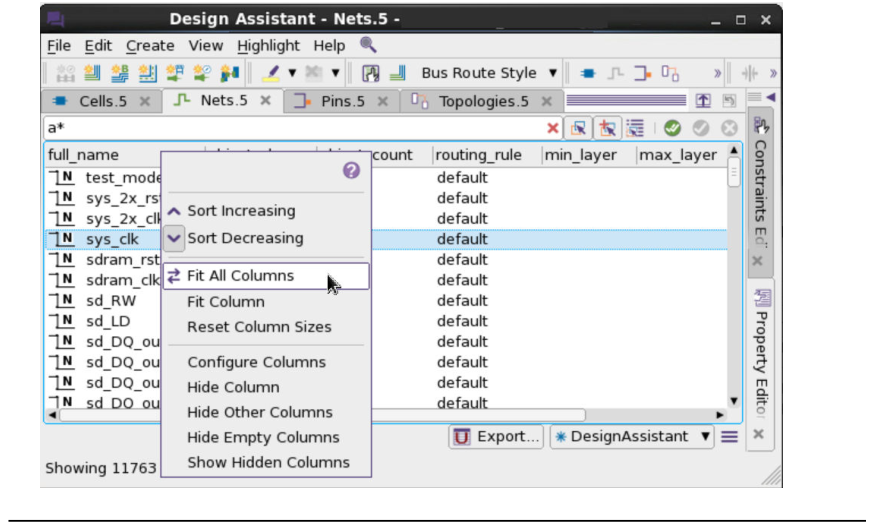
\includegraphics[width=0.92\textwidth]{gui-fig-042.png}
\caption{在设计助手中适配列宽}
\label{fig:gui-42}
\end{figure}

\subsection{更改多个对象的属性设置}
\subsubsection*{Changing Property Settings for Multiple Objects}

可以一次更改多个对象的属性设置。要更改多个所选对象的某项属性：
\begin{enumerate}
  \item 在设计助手中选择多个对象：按住 Shift 键单击表中的各行。也可以按住鼠标并拖动，以选择多行。
  \item 单击某一对象所在的行并更改其值，从而更改该单个对象的属性。
  \item 单击 Apply 按钮，把更改应用到全部所选对象。
\end{enumerate}

见图~\ref{fig:gui-43}。

\begin{figure}[htbp]
\centering
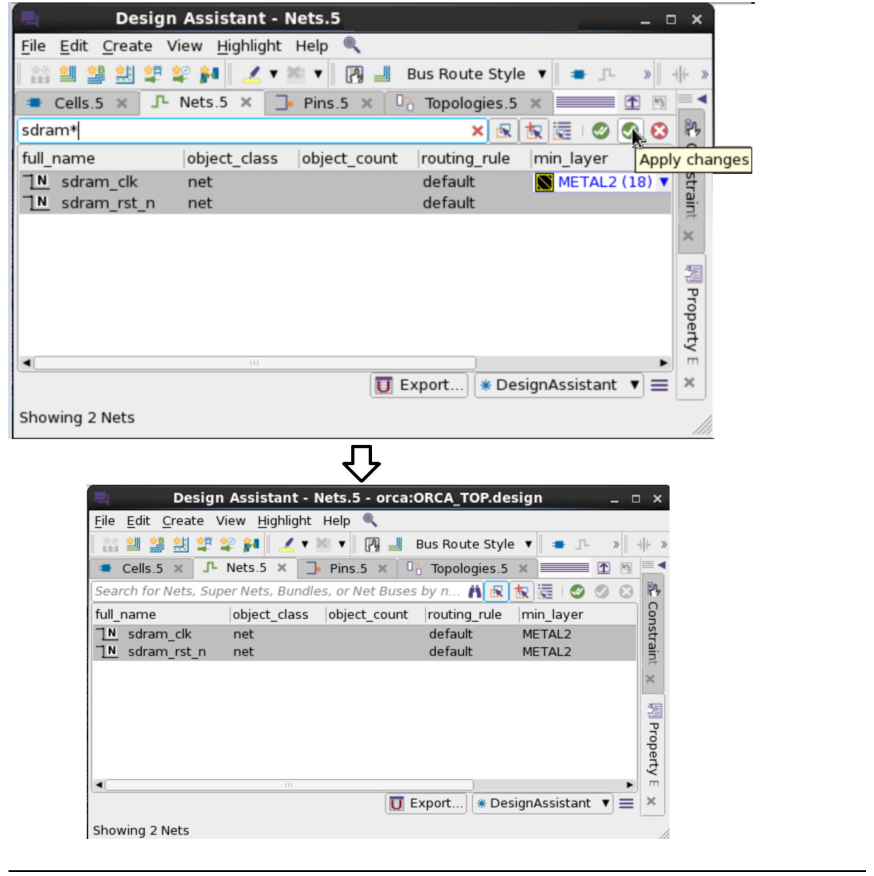
\includegraphics[width=0.92\textwidth]{gui-fig-043.png}
\caption{将更改应用到设计助手中的多个对象}
\label{fig:gui-43}
\end{figure}

\subsection{自动应用更改}
\subsubsection*{Applying the Changes Automatically}

要使更改自动应用到设计，在 Cells、Nets、Pins 和 Topologies 选项卡上单击 Auto Apply Changes，见图~\ref{fig:gui-44}。

\begin{figure}[htbp]
\centering
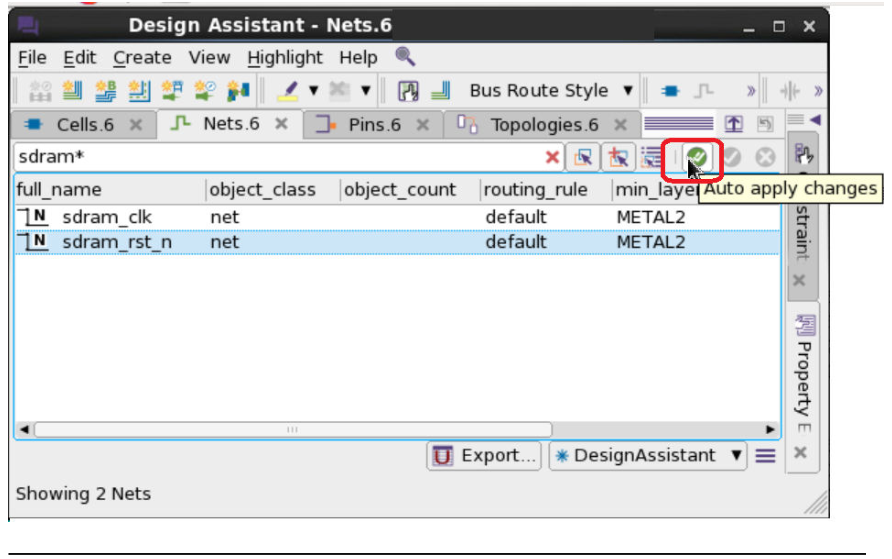
\includegraphics[width=0.92\textwidth]{gui-fig-044.png}
\caption{在设计助手中自动应用更改}
\label{fig:gui-44}
\end{figure}

\subsection{使选择与全局选择同步}
\subsubsection*{Synchronizing the Selection With the Global Selection}

在版图窗口中选择对象时，要使设计助手窗口中对应的对象或行一并被选中，在设计助手窗口的 Cells、Nets、Pins 和 Topologies 选项卡上单击 Synchronize Global Selection 按钮，见图~\ref{fig:gui-45}。

\begin{figure}[htbp]
\centering
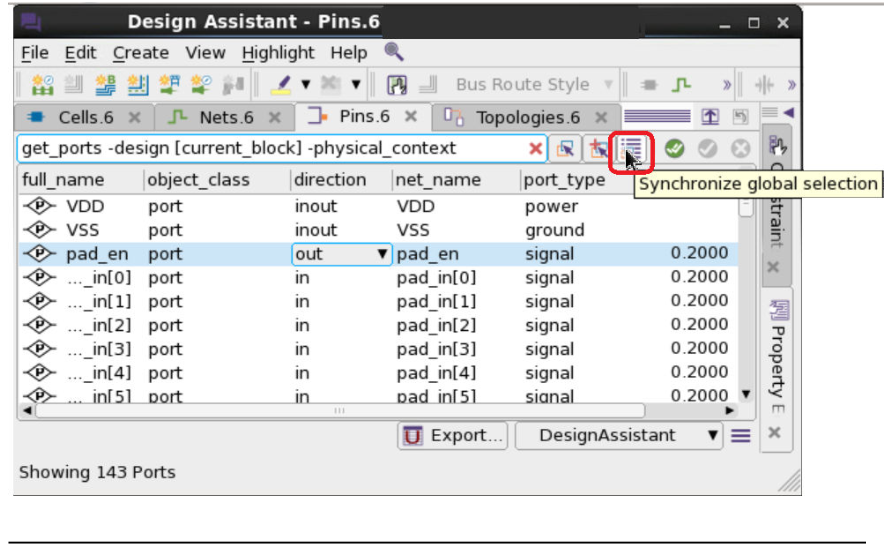
\includegraphics[width=0.92\textwidth]{gui-fig-045.png}
\caption{在设计助手中与全局选择同步}
\label{fig:gui-45}
\end{figure}

\subsection{执行相关任务}
\subsubsection*{Performing Related Tasks}

设计助手窗口中的每个选项卡都支持上下文菜单，其中列出可对对象列表执行的各项任务。把指针移到列表中的一项上，单击鼠标右键即可查看上下文菜单。上下文菜单显示与所选对象相关的任务。例如，在 Cells 选项卡中打开上下文菜单时，菜单会显示所选对象的 \textbf{Get Nets}、\textbf{Get Hierarchical Nets}、\textbf{Get Pins} 和 \textbf{Create Bounds} 任务。单击上下文菜单中的项即可执行该任务。从上下文菜单选择任务后，工具会打开相应选项卡并显示信息。另一个例子是：在 Topologies 选项卡上打开上下文菜单时，菜单会显示所选对象的 \textbf{Get Nets} 任务。要查看或隐藏拓扑规划（topology plan），分别执行 \textbf{Show Topology Plans (hierarchical)} 或 \textbf{Hide Topology Plans} 任务。

\begin{noteBox}
同样的相关操作也可以从菜单栏选择。例如，要显示 Cells 选项卡中所选项目的线网，从设计助手菜单栏选择 \textbf{Cells > Get Nets}。在设计助手中切换不同选项卡时，菜单栏中的项目会随之改变。
\end{noteBox}

也可以用上下文菜单高亮（highlight）对象、放大以查看对象、把用于选择该对象的 Tcl 命令写入脚本文件，以及执行其他任务。单击上下文菜单中的项即可执行相应操作。

\subsection{使用约束编辑器}
\subsubsection*{Using the Constraints Editor}

使用 Constraints Editor 面板显示并修改线网约束、拓扑约束和成形约束（shaping constraint）。线网约束包括与 Nets 选项卡中所选对象关联的非默认布线规则（nondefault routing rule）和布线走廊（routing corridor）。成形约束包括目标位置（target location）、父对象（parent object）、边界（boundary）、利用率（utilization）等，由 \cmd{create\_shaping\_constraint} 命令设置。拓扑约束包括与 Topologies 选项卡上所选拓扑规划关联的拓扑节点（topology node）、拓扑边（topology edge）和中继器（repeater）。

要用该面板查看并修改全部约束：
\begin{enumerate}
  \item 从设计助手菜单选择 \textbf{View > Toolbars > Constraints Editor}，或单击 Constraints Editor 选项卡。
  \item 在 Nets、Topologies 或 Shapeable 视图中选择一个对象。
  \item 单击表中的对象名。
  \item 单击约束列表中的约束类型，查看该约束的属性。
  \item （可选）在属性编辑表中修改该约束的属性。
  \item （可选）在约束表中的约束类型上右键单击，选择 \textbf{Select}、\textbf{Select Owners} 或 \textbf{Delete}，以选择或删除该约束类型。
  \item （可选）单击 Options 按钮（齿轮图标），打开 Synchronize Global Selection 模式，使全局选择与 Constraints Editor 中的选择双向同步。
\end{enumerate}

设计助手视图与 Constraints Editor 调色板（palette）中的该选项互斥，不能同时启用。

要用该面板查看并修改线网约束：
\begin{enumerate}
  \item 从设计助手菜单选择 \textbf{View > Shapeable Objects}。
  \item 从设计助手菜单选择 \textbf{View > Toolbars > Constraints Editor}，或单击 Constraints Editor 选项卡。
  \item 单击表中的对象名。
  \item 单击约束列表中的 [+] 符号，查看该约束的属性。
  \item （可选）在属性编辑表中修改该约束的属性。
  \item （可选）在约束表中的约束类型上单击鼠标右键，选择 \textbf{Select}、\textbf{Select Owners} 或 \textbf{Delete}，以选择或删除该约束类型。
\end{enumerate}

线网约束界面见图~\ref{fig:gui-46}。

\begin{figure}[htbp]
\centering
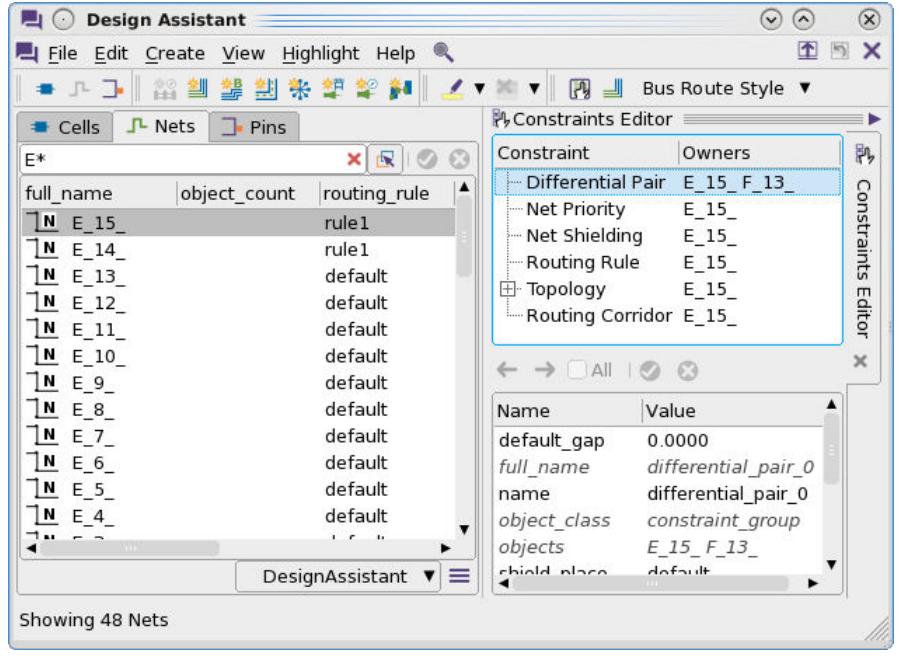
\includegraphics[width=0.92\textwidth]{gui-fig-046.png}
\caption{设计助手的线网约束}
\label{fig:gui-46}
\end{figure}

Constraints Editor 支持基于表达式的过滤和列过滤。单击一条约束并按正斜杠（/）键，即可显示过滤表达式框。也可以在列标题上单击鼠标右键，再单击 Show/Hide Filter Control 按钮，以显示过滤表达式框。在框中输入表达式并按 Enter 键，即可过滤结果。

要做列过滤，单击 Show/Hide column filter control 按钮。工具在每个列标题右侧显示漏斗图标。单击该图标即可显示列过滤菜单，见图~\ref{fig:gui-47}。

\begin{figure}[htbp]
\centering
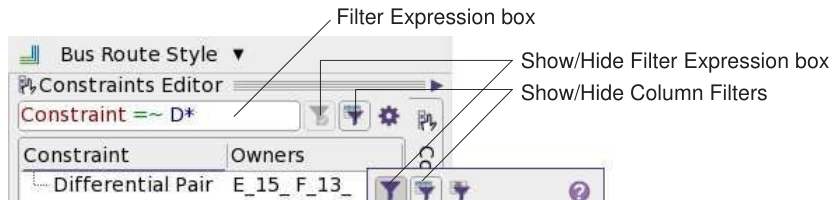
\includegraphics[width=0.92\textwidth]{gui-fig-047.png}
\caption{设计助手的列过滤}
\label{fig:gui-47}
\end{figure}

\subsection{高亮对象}
\subsubsection*{Highlighting Objects}

要在版图中高亮对象，把指针移到列表中的条目上，单击鼠标右键打开上下文菜单，再单击 \textbf{Highlight} 以高亮该对象。也可以在列表中选中对象，然后从设计助手菜单栏选择 \textbf{Highlight > Selected}。要清除某一高亮，选中该对象，并从菜单栏选择 \textbf{Highlight > Clear Selected}。选择 \textbf{Highlight > Clear All} 可清除全部高亮。

\subsection{读写对象选择脚本}
\subsubsection*{Reading and Writing Object Selection Scripts}

要把返回当前选项卡中当前所选对象列表的 Tcl 命令存盘，从菜单栏选择 \textbf{File > Write Script}，或单击鼠标右键并从上下文菜单选择 \textbf{Write Script}。

\begin{noteBox}
执行此操作时，至少要已选中一个对象。
\end{noteBox}

转到要保存文件的目录，输入文件名并单击 Save，即可写出文件。设计助手写出的脚本包含 \cmd{get\_pins}、\cmd{get\_nets} 或 \cmd{get\_cells} 命令，后接当前所选对象的名称。

要从设计助手读取 Tcl 脚本，选择 \textbf{File > Read Script}，或单击鼠标右键并从上下文菜单选择 \textbf{Read Script}。

\section{用相对位置约束工具设置约束}
\subsection*{Setting Constraints With the Relative Location Constraints Tool}

相对位置约束（relative location constraint）工具用于设置、查看和删除硬宏（hard macro）的布局约束。要启动该工具，从菜单选择 \textbf{View > Assistants > Relative Location Constraints}。Relative Location Constraints 面板出现在版图底部，见图~\ref{fig:gui-48}。列表框显示设计中的硬宏实例，以及已指定的相对位置约束。单击列标题可对表排序；再次单击则按相反顺序排序。

\begin{figure}[htbp]
\centering
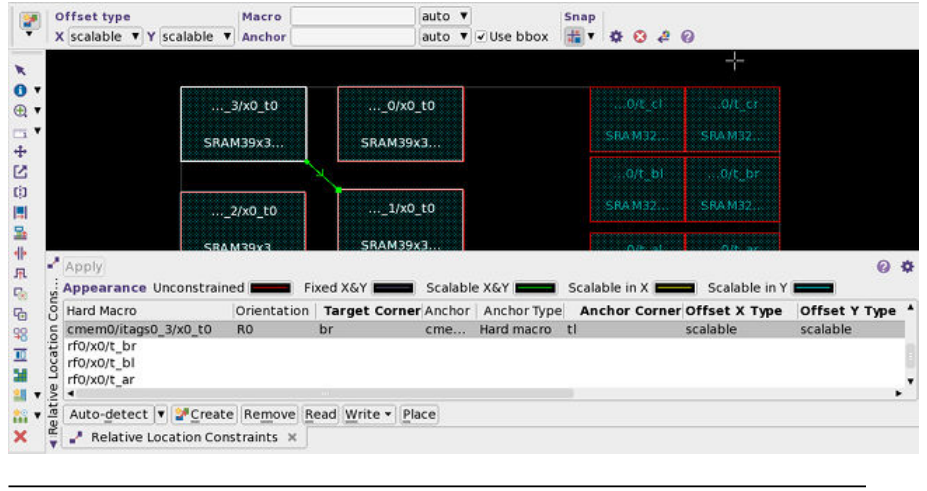
\includegraphics[width=0.92\textwidth]{gui-fig-048.png}
\caption{相对位置约束面板}
\label{fig:gui-48}
\end{figure}

\subsection{手动创建相对位置约束}
\subsubsection*{Manually Creating Relative Location Constraints}

要创建相对位置约束：
\begin{enumerate}
  \item 单击 Create 按钮，开始定义约束。
  \item （可选）按需要在 Mouse Tool Options 工具栏中更改 Offset type 及其他设置。
  \item 单击要约束的目标宏（target macro）的一角，如图~\ref{fig:gui-49} 中的 (1)。
  \item 单击锚点对象（anchor object）的一角，以定义锚点角，如图~\ref{fig:gui-49} 中的 (2)。若难以点中，请确认该锚点对象类型在 View Settings 面板中是可选的。\\
        工具在目标宏与锚点对象的角之间显示约束飞线（constraint flyline），如图~\ref{fig:gui-49} 中的 (3)；Relative Location Constraints 面板中的约束表会更新，以显示这条新约束。
  \item （可选）重复步骤 2 至 4，定义更多宏的相对位置约束。
  \item 按 Esc 退出 Create Macro Relative Location Constraint 工具。
\end{enumerate}

\begin{figure}[htbp]
\centering
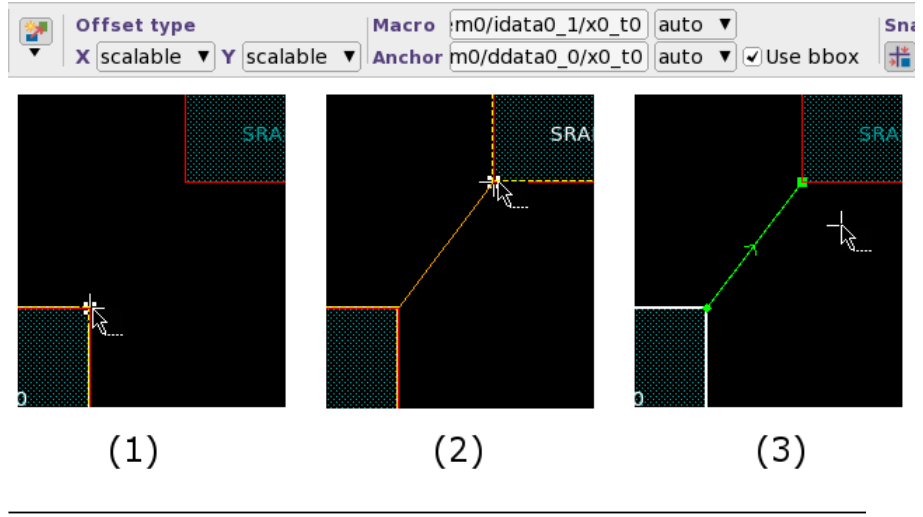
\includegraphics[width=0.92\textwidth]{gui-fig-049.png}
\caption{手动创建相对宏约束}
\label{fig:gui-49}
\end{figure}

\subsection{自动创建相对位置约束}
\subsubsection*{Automatically Creating Relative Location Constraints}

该工具支持自动创建相对位置约束。要为一组所选宏创建约束：
\begin{enumerate}
  \item 用下列方法之一选择一个或多个宏：
  \begin{itemize}
    \item 单击表中的一行。
    \item 单击表中的一行并拖动，以选择多个宏。
    \item 在表中单击，再按 Ctrl+A 选择全部宏。
    \item 在版图中单击一个或多个宏。
  \end{itemize}
  \item 单击 Auto-detect 按钮。\\
        工具为全部所选宏创建相对位置约束。
\end{enumerate}

\subsection{按相对位置约束放置宏}
\subsubsection*{Placing Macros Using Relative Location Constraints}

要按相对位置约束放置宏，单击 Place 按钮，并在出现的对话框中单击 OK。工具运行 \cmd{create\_macro\_relative\_location\_placement} 命令，根据相对位置约束更新宏的布局。

\subsection{删除相对位置约束}
\subsubsection*{Removing Relative Location Constraints}

要删除一条或多条相对位置约束：
\begin{enumerate}
  \item 选择一个或多个宏。
  \item 单击 Remove 按钮以删除约束。
\end{enumerate}

图~\ref{fig:gui-50} 是选中两个宏的约束表。在此例中，单击 Remove 按钮会删除所选宏的约束。

\begin{figure}[htbp]
\centering
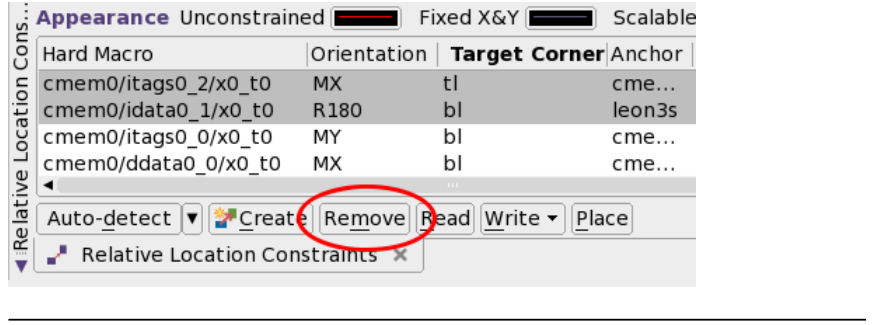
\includegraphics[width=0.92\textwidth]{gui-fig-050.png}
\caption{删除相对位置约束}
\label{fig:gui-50}
\end{figure}

\subsection{写出相对位置约束}
\subsubsection*{Writing Out Relative Location Constraints}

要把已定义约束的全部宏的相对位置约束写出，单击 Write 按钮，选择 Macro relative location，并输入用于保存约束的文件名。对于每个已定义宏相对约束的宏，工具写出一条 \cmd{set\_macro\_relative\_location} 命令。下列示例给出两条已定义的约束：

\begin{lstlisting}
# macro_relative_constraints.tcl
set_macro_relative_location \
   -target_object [get_cells u1/REG_FILE_D_RAM] \
   -target_orientation R0 -target_corner tr \
   -anchor_object [get_blocks ORCA] -anchor_corner tr -offset { \
   -0.1594 -0.2488} -offset_type scalable \
   -used_length {0.0000 0.0000} -scale_edge {0 0}

set_macro_relative_location \
   -target_object [get_cells u2/SD_FIFO_RAM] \
   -target_orientation MXR90 -target_corner br \
   -anchor_object [get_blocks ORCA] -anchor_corner br -offset { \
   -0.1715 0.2576} -offset_type scalable \
   -used_length {0.0000 0.0000} -scale_edge {0 0}

set_attribute -objects [get_blocks test:ORCA.design] \
   -name edge_number -value 4 -quiet
\end{lstlisting}

\subsection{写出端口相对位置约束}
\subsubsection*{Writing Out Port Relative Location Constraints}

要把全部 I/O 端口（I/O port）的端口相对位置约束写出，单击 Write 按钮，选择 Port relative location，并输入用于保存约束的文件名。对于每个已定义相对约束的 I/O 端口，工具写出一条 \cmd{set\_individual\_pin\_constraints} 命令。含有两条已定义约束的设计，其示例文件如下：

\begin{lstlisting}
# Port relative location constraints
# Generated on Feb 3 12:51:21
...
set_individual_pin_constraints -ports [get_ports pad[15]] \
   -sides 2 -offset [mrl_get_offset 2 0.5]
set_individual_pin_constraints -ports [get_ports pad[14]] \
   -sides 2 -offset [mrl_get_offset 2 0.5]
...
\end{lstlisting}

\subsection{读入相对位置约束}
\subsubsection*{Reading In Relative Location Constraints}

要读入宏或 I/O 端口的相对位置约束，单击 Read 按钮，并输入包含宏相对位置约束或 I/O 端口相对位置约束的脚本文件名。工具读取该文件并应用约束。

\subsection{更改约束飞线的颜色}
\subsubsection*{Changing the Color of the Constraint Flylines}

定义了宏相对约束后，工具在宏与对象之间显示约束飞线。要更改约束飞线的颜色：
\begin{enumerate}
  \item 单击面板顶部附近 Appearance 区中的一条色条。
  \item 在 Select Style 对话框中选择新颜色，并单击 OK。
  \item 单击 Apply 以应用更改。
\end{enumerate}

工具用新颜色重新显示约束飞线。

\section{使用网表追踪器}
\subsection*{Using the Netlist Tracer}

IC Compiler II 工具提供网表追踪器（Netlist Tracer），用于追踪一条线网在设计中的路径。从菜单选择 \textbf{View > Assistants > Netlist Tracer} 即可启动网表追踪器。用网表追踪器沿设计遍历线网路径。先选择作为追踪起点的单元、线网、管脚或端口。可以遍历连接到该对象的线网路径，高亮该路径，并放大相关的单元、线网和管脚。追踪路径时，网表追踪器在当前对象与任何相连对象之间显示飞线（flyline）。界面见图~\ref{fig:gui-51}。

\begin{figure}[htbp]
\centering
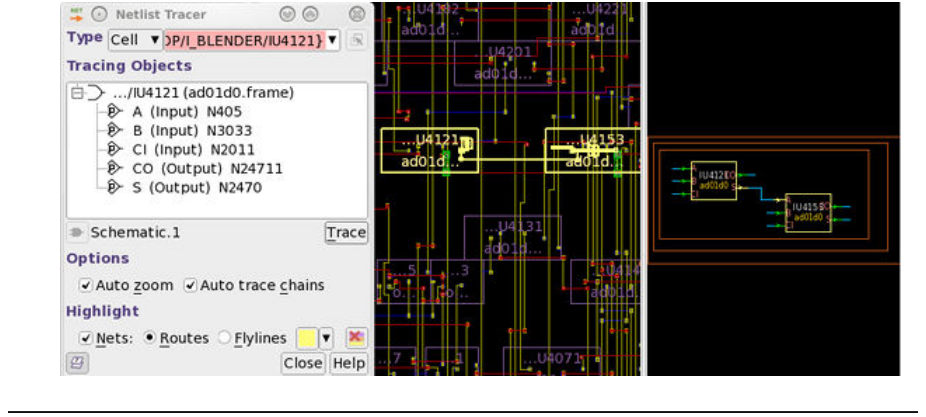
\includegraphics[width=0.92\textwidth]{gui-fig-051.png}
\caption{网表追踪器}
\label{fig:gui-51}
\end{figure}

\section{使用布线轨道助手}
\subsection*{Using the Track Assistant}

用 Track Assistant 面板检查当前设计中的布线轨道（routing track）。布线轨道助手显示所选布线层上轨道的包围盒（bounding box），并显示轨道编号（track number），以表示轨道相对所选区域的位置。可以按层、宽度、首选方向（preferred direction）与非首选方向（nonpreferred direction）以及障碍（obstruction）显示轨道。

要启动布线轨道助手，从菜单选择 \textbf{View > Assistants > Track Assistant}，或单击 Track Assistant 按钮。以下几节说明如何使用布线轨道助手。面板见图~\ref{fig:gui-52}。

\begin{figure}[htbp]
\centering
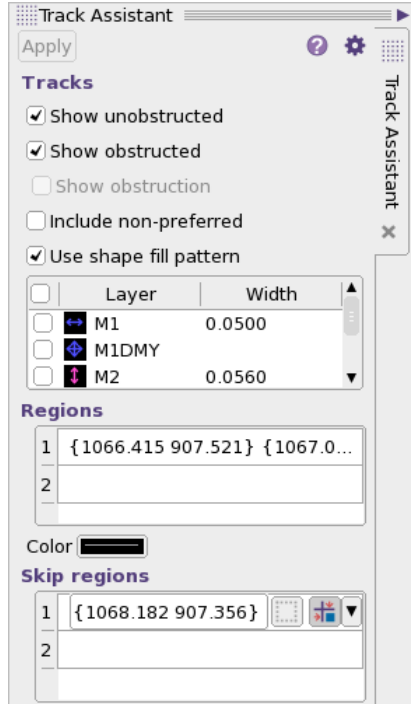
\includegraphics[width=0.92\textwidth]{gui-fig-052.png}
\caption{布线轨道助手}
\label{fig:gui-52}
\end{figure}

\subsection{显示轨道}
\subsubsection*{Displaying Tracks}

要用布线轨道助手显示轨道：
\begin{enumerate}
  \item 从菜单选择 \textbf{View > Assistants > Track Assistant}，启动布线轨道助手。
  \item 放大到要检查的版图区域。
  \item 选择要显示轨道的层。\\
        工具按所选层的轨道宽度显示布线轨道，见图~\ref{fig:gui-53}。默认情况下，工具同时显示畅通轨道与受阻轨道。
\end{enumerate}

\begin{figure}[htbp]
\centering
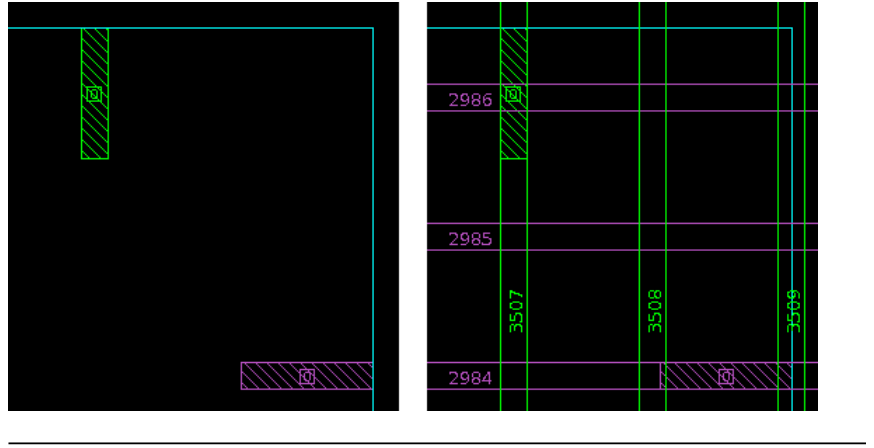
\includegraphics[width=0.92\textwidth]{gui-fig-053.png}
\caption{显示轨道之前与之后}
\label{fig:gui-53}
\end{figure}

\subsection{在指定区域显示轨道信息}
\subsubsection*{Displaying Track Information in Specific Regions}

用布线轨道助手中的选项，可以把轨道显示限制在设计的指定区域。要只显示设计中某些区域的轨道信息：
\begin{enumerate}
  \item 按上一节所述启动布线轨道助手并选择层。
  \item 在 Regions 区的空行中单击，并输入要显示区域的包围盒。\\
        也可以单击 Specify Rectangle 按钮，在版图上画出该区域。要清除区域，把鼠标指针移到面板中的包围盒坐标上，并单击 Clear region 按钮。
  \item （可选）按需要重复上一步，画出更多区域。
  \item （可选）在 Skip regions 区的空行中单击，并输入该区域的包围盒，以创建一个隐藏轨道显示的区域。\\
        也可以单击 Specify Rectangle 按钮，在版图上画出跳过区域（skip region）。
\end{enumerate}

图~\ref{fig:gui-54} 是版图与布线轨道助手面板，其中只显示一个指定区域以及一个跳过区域。

\begin{noteBox}
已定义区域之外不显示轨道。
\end{noteBox}

\begin{figure}[htbp]
\centering
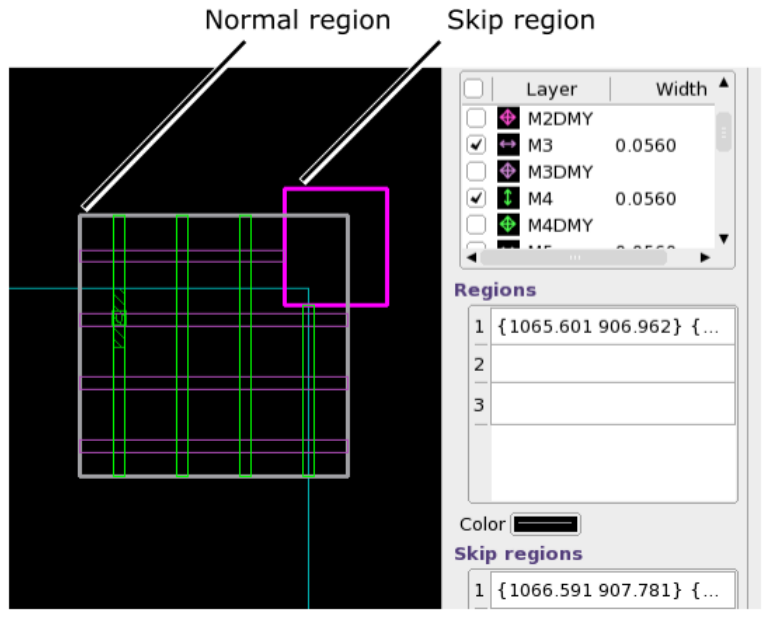
\includegraphics[width=0.92\textwidth]{gui-fig-054.png}
\caption{带普通区域与跳过区域的布线轨道助手}
\label{fig:gui-54}
\end{figure}

\subsection{显示受阻或畅通的轨道}
\subsubsection*{Displaying Obstructed or Unobstructed Tracks}

启动布线轨道助手时，工具同时显示受阻轨道（obstructed track）与畅通轨道（unobstructed track）。要只显示畅通轨道，选中 Show unobstructed 选项，并取消选中 Show obstructed 选项。要只显示受阻轨道，取消选中 Show unobstructed 选项，并选中 Show obstructed 选项。要高亮障碍，选中 Show obstruction 选项。

图~\ref{fig:gui-55} 是显示受阻轨道时的面板设置与版图。

\begin{figure}[htbp]
\centering
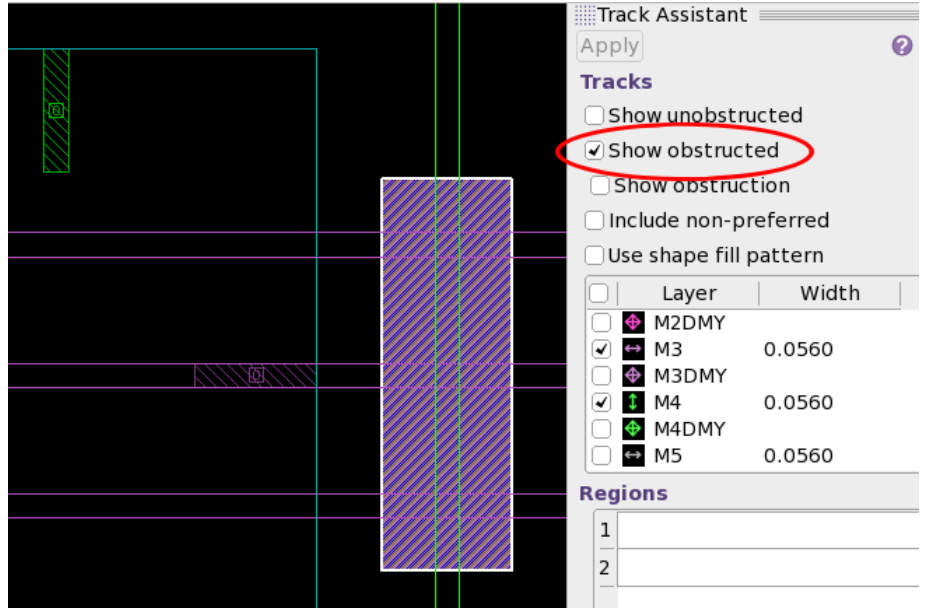
\includegraphics[width=0.92\textwidth]{gui-fig-055.png}
\caption{受阻轨道}
\label{fig:gui-55}
\end{figure}

\subsection{设置布线轨道助手选项}
\subsubsection*{Setting Track Assistant Options}

Track Assistant 面板还支持下列选项：
\begin{itemize}
  \item 选择 Include non-preferred 选项，同时显示首选布线方向与非首选布线方向上的轨道。
  \item 选择 Use shape fill pattern 选项，使布线轨道使用与金属层相同的填充图案。
  \item 单击区域列表下方的色条，并在 Select Style 对话框中选择新颜色，以设置普通区域或跳过区域的颜色。
\end{itemize}
